\documentclass{beamer}
\usetheme{Darmstadt}
\definecolor{dgrey}{rgb}{0.25, 0.25, 0.25}
\usecolortheme[named=dgrey]{structure}

\usepackage[utf8]{inputenc}
\usepackage{graphicx}
\usepackage{multicol}
\usepackage{xcolor}

\definecolor{dgreen}{HTML}{005500}
\definecolor{dblue}{HTML}{000088}
\definecolor{dred}{HTML}{BB0000}

\renewcommand{\.}{\hskip .75pt}

\DeclareMathOperator{\aand}{~\wedge~}
\DeclareMathOperator{\conv}{conv}
\DeclareMathOperator{\rank}{rank}

\newcommand\Wider[2][3em]{
	\makebox[\linewidth][c]{
		\begin{minipage}{\dimexpr\textwidth+#1\relax}
			\raggedright#2
		\end{minipage}
	}
}


\title{Computer Science Track Core Course}
\subtitle{Linear programming --- recitation 2}
\author{Martin Dvorak\\ISTA\\Kolmogorov group}
\date{2023-05-16}



\begin{document}

\begin{frame}
 	\titlepage
\end{frame}


\begin{frame}
	\frametitle{Linear equalities versus inequalities}
	\framesubtitle{Remark about Rouché-Capelli theorem}
	
	\begin{columns} 
		\begin{column}{0.55\textwidth}
			\;\;\,\, We have $A \in \mathbb{R}^{m \times n}$ and	$b \in \mathbb{R}^{m}$.
		\end{column}
	
		\begin{column}{0.5\textwidth}
			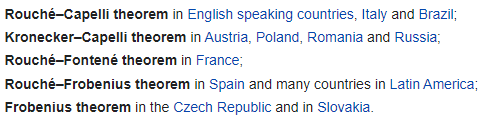
\includegraphics[width=\textwidth]{Rouche_wiki}
		\end{column}
	\end{columns}
	
	
	\smallskip
	
	{ \color{dred}
		Rouché-Capelli theorem for the system of equalities $A\. \bold{x} = b$ \dots
		
		Exactly one of the following statements is true:
	}
	\begin{itemize} \color{dred}
		\item $\exists \bold{x} \in \mathbb{R}^{n} : \ \; A\. \bold{x} = b$
		\item $\exists \bold{y} \in \mathbb{R}^{m} : \ \; A^{\!\top} \bold{y} = \bold{0} \aand b^{\!\top} \bold{y} \alt<2>{<}{\neq} 0$
	\end{itemize}
	\bigskip
	
	Rouché-Capelli theorem is typically stated as\,\dots
	
	Let $A \in F^{m \times n}$ be a matrix and $b \in F^{m}$ be a vector over a field $F$.
	
	The system of equalities $A\. \bold{x} = b$ is \textcolor{dgreen}{inconsistent} (that is, no solution $\bold{x} \in F^{n}$ exists) \textcolor{dgreen}{if and only if} $\rank(A) < \rank(A\,|b)$.

\end{frame}


\begin{frame}
	\frametitle{Linear equalities versus inequalities}
	\framesubtitle{Rouché-Capelli theorem versus Farkas' lemma (I)}
	
	Now we fix $A \in \mathbb{R}^{m \times n}$ and $b \in \mathbb{R}^{m}$.
	\bigskip
	
	{ \color{dred}
		Rouché-Capelli theorem for the system of equalities $A\. \bold{x} = b$ \dots
		
		Exactly one of the following statements is true:
	}
	\begin{itemize} \color{dred}
		\item $\exists \bold{x} \in \mathbb{R}^{n} : \ \; A\. \bold{x} = b$ \hfill\hbox{\footnotesize(*)\:\qquad}
		\item $\exists \bold{y} \in \mathbb{R}^{m} : \ \; A^{\!\top} \bold{y} = \bold{0} \aand b^{\!\top} \bold{y} \neq 0$ \hfill\hbox{\footnotesize(**)\qquad}
	\end{itemize}
	\medskip
	
	{ \color{dblue}
		Farkas' lemma for the system of equalities $A\. \bold{x} = b$ \.over \.$\bold{x} \ge 0$\,\dots
		
		Exactly one of the following statements is true:
	}
	\begin{itemize} \color{dblue}
		\item $\exists \bold{x} \in \mathbb{R}^{n} : \ \; A\. \bold{x} = b \aand \bold{x} \ge \bold{0}$ \hfill\hbox{\footnotesize(*)\:\qquad}
		\item $\exists \bold{y} \in \mathbb{R}^{m} : \ \; A^{\!\top} \bold{y} \ge \bold{0} \aand b^{\!\top} \bold{y} < 0$ \hfill\hbox{\footnotesize(**)\qquad}
	\end{itemize}
	\medskip
	
	\footnotesize Intuition behind the dichotomy:\qquad
	(*) The problem has a solution.

	(**) There is a linear combination of rows that provides a contradiction.
	
\end{frame}


\begin{frame}
	\frametitle{Linear equalities versus inequalities}
	\framesubtitle{Rouché-Capelli theorem versus Farkas' lemma (II)}
	
	Now we fix $A \in \mathbb{R}^{m \times n}$ and $b \in \mathbb{R}^{m}$.
	\bigskip
	
	{ \color{dred}
		Rouché-Capelli theorem for the system of equalities $A\. \bold{x} = b$ \dots
		
		Exactly one of the following statements is true:
	}
	\begin{itemize} \color{dred}
		\item $\exists \bold{x} \in \mathbb{R}^{n} : \ \; A\. \bold{x} = b$ \hfill\hbox{\footnotesize(*)\:\qquad}
		\item $\exists \bold{y} \in \mathbb{R}^{m} : \ \; A^{\!\top} \bold{y} = \bold{0} \aand b^{\!\top} \bold{y} \neq 0$ \hfill\hbox{\footnotesize(**)\qquad}
	\end{itemize}
	\medskip
	
	{ \color{dblue}
		Farkas' lemma for the system of inequalities $A\. \bold{x} \le b$, $\bold{x} \lessgtr 0$ \dots
		
		Exactly one of the following statements is true:
	}
	\begin{itemize} \color{dblue}
		\item $\exists \bold{x} \in \mathbb{R}^{n} : \ \; A\. \bold{x} \le b$ \hfill\hbox{\footnotesize(*)\:\qquad}
		\item $\exists \bold{y} \in \mathbb{R}^{m} : \ \; A^{\!\top} \bold{y} = \bold{0} \aand b^{\!\top} \bold{y} < 0 \aand \bold{y} \ge \bold{0}$ \hfill\hbox{\footnotesize(**)\qquad}
	\end{itemize}
	\medskip
	
	\footnotesize Intuition behind the dichotomy:\qquad
	(*) The problem has a solution.
	
	(**) There is a linear/nnlin.~combination of rows that provides a contradiction.

\end{frame}


\begin{frame}
\frametitle{Linear equalities versus inequalities}
\framesubtitle{Rouché-Capelli theorem versus Farkas' lemma (III)}

	Now we fix $A \in \mathbb{R}^{m \times n}$ and $b \in \mathbb{R}^{m}$.
	\bigskip
	
	{ \color{dred}
		Rouché-Capelli theorem for the system of equalities $A\. \bold{x} = b$ \dots
		
		Exactly one of the following statements is true:
	}
	\begin{itemize} \color{dred}
		\item $\exists \bold{x} \in \mathbb{R}^{n} : \ \; A\. \bold{x} = b$ \hfill\hbox{\footnotesize(*)\:\qquad}
		\item $\exists \bold{y} \in \mathbb{R}^{m} : \ \; A^{\!\top} \bold{y} = \bold{0} \aand b^{\!\top} \bold{y} \neq 0$ \hfill\hbox{\footnotesize(**)\qquad}
	\end{itemize}
	\medskip
	
	{ \color{dblue}
		Farkas' lemma for the system of inequalities $A\. \bold{x} \le b$, $\bold{x} \ge 0$ \dots
		
		Exactly one of the following statements is true:
	}
	\begin{itemize} \color{dblue}
		\item $\exists \bold{x} \in \mathbb{R}^{n} : \ \; A\. \bold{x} \le b \aand \bold{x} \ge \bold{0}$ \hfill\hbox{\footnotesize(*)\:\qquad}
		\item $\exists \bold{y} \in \mathbb{R}^{m} : \ \; A^{\!\top} \bold{y} \ge \bold{0} \aand b^{\!\top} \bold{y} < 0 \aand \bold{y} \ge \bold{0}$ \hfill\hbox{\footnotesize(**)\qquad}
	\end{itemize}
	\medskip
	
	\footnotesize Intuition behind the dichotomy:\qquad
	(*) The problem has a solution.
	
	(**) There is a linear/nnlin.~combination of rows that provides a contradiction.

\end{frame}


\begin{frame}
	\frametitle{Linear equalities versus inequalities}
	\framesubtitle{Summary of Farkas' lemmata}
	
	We have $A \in \mathbb{R}^{m \times n}$ and $b \in \mathbb{R}^{m}$.
	\smallskip
	
	Exactly one of the following statements is true:\vspace{-1mm}
	\begin{itemize} \color{dblue}
		\item $\exists \bold{x} \in \mathbb{R}^{n} : \ \; A\. \bold{x} = b \aand \bold{x} \ge \bold{0}$
		\item $\exists \bold{y} \in \mathbb{R}^{m} : \ \; A^{\!\top} \bold{y} \ge \bold{0} \aand b^{\!\top} \bold{y} < 0$
	\end{itemize}
		
	Exactly one of the following statements is true:\vspace{-1mm}
	\begin{itemize} \color{dblue}
		\item $\exists \bold{x} \in \mathbb{R}^{n} : \ \; A\. \bold{x} \le b$
		\item $\exists \bold{y} \in \mathbb{R}^{m} : \ \; A^{\!\top} \bold{y} = \bold{0} \aand b^{\!\top} \bold{y} < 0 \aand \bold{y} \ge \bold{0}$
	\end{itemize}

	Exactly one of the following statements is true:\vspace{-1mm}
	\begin{itemize} \color{dblue}
		\item $\exists \bold{x} \in \mathbb{R}^{n} : \ \; A\. \bold{x} \le b \aand \bold{x} \ge \bold{0}$
		\item $\exists \bold{y} \in \mathbb{R}^{m} : \ \; A^{\!\top} \bold{y} \ge \bold{0} \aand b^{\!\top} \bold{y} < 0 \aand \bold{y} \ge \bold{0}$
	\end{itemize}
	\smallskip

	Farkas' lemmata have many applications.
	
	Their staple use case is the proof of the Strong duality theorem(s).
	
\end{frame}


\begin{frame}
	\frametitle{Strong duality}
	\framesubtitle{Let's outline the proof for the bounded case using Farkas' lemma (III)}
	
	We have $E \in \mathbb{R}^{m \times n}$ and $d \in \mathbb{R}^{m}$.
	\smallskip

	Exactly one of the following statements is true:
	\begin{itemize} \color{dblue}
		\item $\exists \bold{w} \in \mathbb{R}^{n} : \ \; E\. \bold{w} \le d \aand \bold{w} \ge \bold{0}$
		\item $\exists \bold{z} \in \mathbb{R}^{m} : \ \; E^{\!\top} \bold{z} \ge \bold{0} \aand d^{\!\top} \bold{z} < 0 \aand \bold{z} \ge \bold{0}$
	\end{itemize}
	\bigskip

	LP duality (III):
	\bigskip

	\begin{columns} 
		\begin{column}{0.5\textwidth}
		\qquad 
		Primal problem:
		$$
		\begin{array}{lrcrcl}
			\text{minimize} & c^{\!\top}\bold{x} \\
			\text{s.\.t.} & A\. \bold{x} \ge b \\
			\text{where} & \bold{x} \ge \bold{0}
		\end{array}
		$$
		\end{column}
		
		\begin{column}{0.5\textwidth}
		\quad~
		Dual problem:
		$$
		\begin{array}{lrcrcl}
			\text{maximize} & b^{\!\top}\bold{y} \\
			\text{s.\.t.} & A^{\!\top} \bold{y} \le c \\
			\text{where} & \bold{y} \ge \bold{0}
		\end{array}
		$$
		\end{column}
	\end{columns}
	
\end{frame}


\begin{frame}
	\frametitle{Systems of linear equalities versus inequalities}
	\framesubtitle{Complexity over rationals versus integers}

	\onslide<2->{{\color{dgreen}Green color} denotes that the problem can be solved in deterministic polynomial time.} \bigskip
	\bigskip
	
	\begin{tabular}{ | c | c | c | }
		\hline
		Domain & Equalities & Inequalities \\
		\hline
		$\mathbb{Q}^n$ & \onslide<2->{\color{dgreen}{Gaussian elimination}} & \onslide<3->{\color{dgreen}{Ellipsoid method}} \\ 
		\hline
		$\mathbb{Z}^n$ & \onslide<4->{\color{dgreen}{Hermite normal form}} & \onslide<5->{\color{dred}{NP-complete}} \\
		\hline
	\end{tabular}
	\bigskip
	\bigskip
	
	\onslide<6->{Exercise: Construct a polynomial reduction from {\color{dred}3-SAT} to {\color{dred}ILP}.}
	
\end{frame}


\end{document}